\section{距离协方差}
\label{sec:dep-distance-covariance}

互信息不看取值之间的距离，也没有有限上界。对欧氏空间中的随机向量，我们想要另一种度量：它的零值仍然刻画独立，数值又能用成对距离直接计算，并且有界。出发点是第~\ref{chap:weak-convergence-of-distributions}章的特征函数。设$\bm{X}$取值于$\mathbb{R}^{p}$，$\bm{Y}$取值于$\mathbb{R}^{q}$，联合特征函数为
\[
  \phi_{\bm{X},\bm{Y}}(\bm{t},\bm{s})=\mathbb{E}\bigl[\mathrm{e}^{\mathrm{i}\langle\bm{t},\bm{X}\rangle+\mathrm{i}\langle\bm{s},\bm{Y}\rangle}\bigr],\qquad \bm{t}\in\mathbb{R}^{p},\ \bm{s}\in\mathbb{R}^{q}.
\]
边缘乘积$P_{\bm{X}}\otimes P_{\bm{Y}}$的特征函数是$\phi_{\bm{X}}(\bm{t})\phi_{\bm{Y}}(\bm{s})$：在乘积空间上取独立的$\tilde{\bm{X}}\sim P_{\bm{X}}$、$\tilde{\bm{Y}}\sim P_{\bm{Y}}$，期望分解成乘积。特征函数确定分布，所以独立等价于两个特征函数处处相等。依赖的大小就用它们之差
\[
  \Delta(\bm{t},\bm{s})=\phi_{\bm{X},\bm{Y}}(\bm{t},\bm{s})-\phi_{\bm{X}}(\bm{t})\,\phi_{\bm{Y}}(\bm{s})
\]
在所有频率上的加权平方积分来量。关键在于选什么权重。

\subsection{定义与独立性}
\label{sec:dep-dcov-definition}

权重要满足三点：处处为正，才不会漏掉某个频段的差别；积分有限；最好还能把积分算回原来的取值空间。下面这个积分恒等式说明，幂次权重$\lVert\bm{t}\rVert_2^{-(d+1)}$把“频率空间里的$1-\cos$”变成“取值空间里的距离”。

\begin{lemma}[余弦积分与距离]
\label{lem:dep-cos-integral}
对$d\geq1$，记
\begin{equation}
  c_d=\int_{\mathbb{R}^{d}}\frac{1-\cos t_1}{\lVert\bm{t}\rVert_2^{d+1}}\,\mathrm{d}\bm{t},
  \label{eq:dep-cd}
\end{equation}
其中$t_1$是$\bm{t}$的第一个坐标。则$0<c_d<\infty$，$c_1=\pi$，并且对每个$\bm{x}\in\mathbb{R}^{d}$，
\begin{equation}
  \int_{\mathbb{R}^{d}}\frac{1-\cos\langle\bm{t},\bm{x}\rangle}{\lVert\bm{t}\rVert_2^{d+1}}\,\mathrm{d}\bm{t}=c_d\,\lVert\bm{x}\rVert_2 .
  \label{eq:dep-cos-integral}
\end{equation}
\end{lemma}

\begin{proof}
先证式~\eqref{eq:dep-cd}有限。在单位球内，
\[
  1-\cos t_1\leq\tfrac12t_1^{2}\leq\tfrac12\lVert\bm{t}\rVert_2^{2},
\]
被积函数不超过$\frac12\lVert\bm{t}\rVert_2^{1-d}$。用极坐标，$\mathbb{R}^{d}$中半径$r$的球面面积与$r^{d-1}$成正比，
\[
  \int_{\lVert\bm{t}\rVert_2\leq1}\lVert\bm{t}\rVert_2^{1-d}\,\mathrm{d}\bm{t}\ \propto\ \int_0^1r^{1-d}\,r^{d-1}\,\mathrm{d}r=1 .
\]
在单位球外，由$1-\cos t_1\leq2$，被积函数不超过$2\lVert\bm{t}\rVert_2^{-d-1}$，对应的径向积分为$\int_1^\infty r^{-2}\,\mathrm{d}r=1$。两部分都有限。被积函数非负，且在$t_1\notin2\pi\mathbb{Z}$处为正，所以$c_d>0$。

再证式~\eqref{eq:dep-cos-integral}。$\bm{x}=\bm{0}$时两边都是零。$\bm{x}\neq\bm{0}$时，取正交矩阵$\bm{R}$使$\bm{R}\bm{x}=\lVert\bm{x}\rVert_2\bm{e}_1$，作代换$\bm{u}=\bm{R}\bm{t}$。正交变换保持体积与范数，并且
\[
  \langle\bm{t},\bm{x}\rangle=\langle\bm{R}\bm{t},\bm{R}\bm{x}\rangle=\lVert\bm{x}\rVert_2u_1 ,
\]
所以左边变为
\[
  \int_{\mathbb{R}^{d}}\frac{1-\cos(\lVert\bm{x}\rVert_2u_1)}{\lVert\bm{u}\rVert_2^{d+1}}\,\mathrm{d}\bm{u}.
\]
再令$\bm{v}=\lVert\bm{x}\rVert_2\bm{u}$，体积元与分母分别变为
\[
  \mathrm{d}\bm{u}=\lVert\bm{x}\rVert_2^{-d}\,\mathrm{d}\bm{v},\qquad \lVert\bm{u}\rVert_2^{d+1}=\lVert\bm{x}\rVert_2^{-d-1}\lVert\bm{v}\rVert_2^{d+1},
\]
积分变为
\[
  \lVert\bm{x}\rVert_2^{d+1}\cdot\lVert\bm{x}\rVert_2^{-d}\int_{\mathbb{R}^{d}}\frac{1-\cos v_1}{\lVert\bm{v}\rVert_2^{d+1}}\,\mathrm{d}\bm{v}=c_d\,\lVert\bm{x}\rVert_2 .
\]

最后求$c_1$。三角形密度$f(x)=(1-\lvert x\rvert)^{+}$的特征函数是
\[
  \phi(t)=2\int_0^1(1-x)\cos(tx)\,\mathrm{d}x=\frac{2(1-\cos t)}{t^{2}},
\]
最后一步用分部积分：
\[
  \int_0^1(1-x)\cos(tx)\,\mathrm{d}x=\Bigl[(1-x)\frac{\sin tx}{t}\Bigr]_0^1+\int_0^1\frac{\sin tx}{t}\,\mathrm{d}x=\frac{1-\cos t}{t^{2}}.
\]$\phi$非负可积，由第~\ref{chap:weak-convergence-of-distributions}章的反演公式在$x=0$处，
\[
  1=f(0)=\frac{1}{2\pi}\int_{-\infty}^{\infty}\phi(t)\,\mathrm{d}t=\frac1\pi\int_{-\infty}^{\infty}\frac{1-\cos t}{t^{2}}\,\mathrm{d}t ,
\]
所以$c_1=\pi$。
\end{proof}

一般维数的常数是$c_d=\pi^{(d+1)/2}/\Gamma\bigl((d+1)/2\bigr)$，后面只用到它有限且为正，不需要具体数值。图~\ref{fig:dep-cos-kernel}画出$d=1$的被积函数：$x=2$的曲线在原点附近高出四倍、宽度减半，总面积恰好加倍。

\begin{BookInlineFigure}
  \centering
  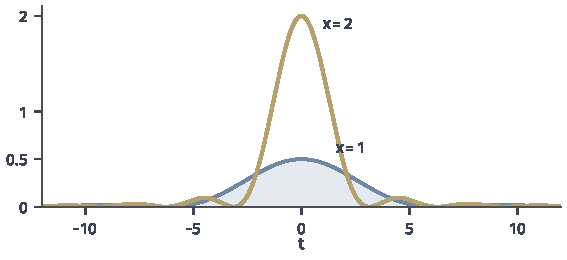
\includegraphics[width=96mm]{figures/07-probability/04-distribution-analysis/matplotlib/dep-cos-kernel/figure.pdf}
  \caption{引理~\ref{lem:dep-cos-integral}在$d=1$时的被积函数$(1-\cos tx)/t^{2}$。蓝线与浅蓝面积对应$x=1$，黄线对应$x=2$；两者在实轴上的积分分别为$\pi$与$2\pi$，与$\lvert x\rvert$成正比（数值积分在$[-4000,4000]$上得$3.1401$与$6.2787$，截去的尾部不超过$2/4000$与$4/4000$）。}
  \label{fig:dep-cos-kernel}
\end{BookInlineFigure}

现在用这个权重定义距离协方差。

\begin{definition}[距离协方差]
\label{def:dep-dcov}
设$\bm{X}\in\mathbb{R}^{p}$、$\bm{Y}\in\mathbb{R}^{q}$满足$\mathbb{E}\lVert\bm{X}\rVert_2<\infty$、$\mathbb{E}\lVert\bm{Y}\rVert_2<\infty$。$\bm{X}$与$\bm{Y}$的\term{距离协方差}（distance covariance）的平方定义为
\begin{equation}
  \operatorname{dCov}^{2}(\bm{X},\bm{Y})=\frac{1}{c_pc_q}\int_{\mathbb{R}^{p+q}}\frac{\lvert\Delta(\bm{t},\bm{s})\rvert^{2}}{\lVert\bm{t}\rVert_2^{p+1}\lVert\bm{s}\rVert_2^{q+1}}\,\mathrm{d}\bm{t}\,\mathrm{d}\bm{s},
  \label{eq:dep-dcov-def}
\end{equation}
其中$\Delta$是联合特征函数与边缘特征函数乘积之差。它的非负平方根记为$\operatorname{dCov}(\bm{X},\bm{Y})$。
\end{definition}

被积函数非负，积分总有意义，下面的定理说明一阶矩条件保证它有限，并且零值恰好刻画独立。

\begin{theorem}[距离协方差的有限性与零值]
\label{thm:dep-dcov-independence}
在定义~\ref{def:dep-dcov}的条件下，设$\bm{X}'$是$\bm{X}$的独立复制，$\bm{Y}'$是$\bm{Y}$的独立复制。则
\begin{equation}
  0\leq\operatorname{dCov}^{2}(\bm{X},\bm{Y})\leq\mathbb{E}\lVert\bm{X}-\bm{X}'\rVert_2\ \mathbb{E}\lVert\bm{Y}-\bm{Y}'\rVert_2<\infty ,
  \label{eq:dep-dcov-bound}
\end{equation}
并且$\operatorname{dCov}^{2}(\bm{X},\bm{Y})=0$当且仅当$\bm{X}$与$\bm{Y}$独立。
\end{theorem}

\begin{proof}
\emph{有限性。}把$\Delta$写成两个中心化复指数乘积的期望。展开右边并逐项取期望，
\[
  \mathbb{E}\Bigl[\bigl(\mathrm{e}^{\mathrm{i}\langle\bm{t},\bm{X}\rangle}-\phi_{\bm{X}}(\bm{t})\bigr)\bigl(\mathrm{e}^{\mathrm{i}\langle\bm{s},\bm{Y}\rangle}-\phi_{\bm{Y}}(\bm{s})\bigr)\Bigr]=\phi_{\bm{X},\bm{Y}}-\phi_{\bm{X}}\phi_{\bm{Y}}-\phi_{\bm{Y}}\phi_{\bm{X}}+\phi_{\bm{X}}\phi_{\bm{Y}},
\]
右边正是$\Delta(\bm{t},\bm{s})$。对复值随机变量用Cauchy--Schwarz不等式
\[
  \lvert\mathbb{E}[UV]\rvert^{2}\leq\mathbb{E}\lvert U\rvert^{2}\,\mathbb{E}\lvert V\rvert^{2},
\]
并注意
\[
  \mathbb{E}\bigl\lvert\mathrm{e}^{\mathrm{i}\langle\bm{t},\bm{X}\rangle}-\phi_{\bm{X}}(\bm{t})\bigr\rvert^{2}=1-\lvert\phi_{\bm{X}}(\bm{t})\rvert^{2},
\]
得到
\[
  \lvert\Delta(\bm{t},\bm{s})\rvert^{2}\leq\bigl(1-\lvert\phi_{\bm{X}}(\bm{t})\rvert^{2}\bigr)\bigl(1-\lvert\phi_{\bm{Y}}(\bm{s})\rvert^{2}\bigr).
\]
右边分离了$\bm{t}$与$\bm{s}$。用独立复制$\bm{X}'$把共轭$\overline{\phi_{\bm{X}}(\bm{t})}$写成$\mathbb{E}\,\mathrm{e}^{-\mathrm{i}\langle\bm{t},\bm{X}'\rangle}$，再取实部，
\[
  1-\lvert\phi_{\bm{X}}(\bm{t})\rvert^{2}=1-\mathbb{E}\,\mathrm{e}^{\mathrm{i}\langle\bm{t},\bm{X}-\bm{X}'\rangle}=\mathbb{E}\bigl[1-\cos\langle\bm{t},\bm{X}-\bm{X}'\rangle\bigr].
\]被积函数非负，由Tonelli定理交换积分与期望，再用引理~\ref{lem:dep-cos-integral}，
\[
  \int_{\mathbb{R}^{p}}\frac{1-\lvert\phi_{\bm{X}}(\bm{t})\rvert^{2}}{\lVert\bm{t}\rVert_2^{p+1}}\,\mathrm{d}\bm{t}=c_p\,\mathbb{E}\lVert\bm{X}-\bm{X}'\rVert_2 .
\]
$\bm{Y}$一侧同理。两式相乘再除以$c_pc_q$，就是式~\eqref{eq:dep-dcov-bound}。由三角不等式，$\mathbb{E}\lVert\bm{X}-\bm{X}'\rVert_2$不超过$2\,\mathbb{E}\lVert\bm{X}\rVert_2<\infty$。

\emph{零值。}若$\bm{X},\bm{Y}$独立，则$\mathrm{e}^{\mathrm{i}\langle\bm{t},\bm{X}\rangle}$与$\mathrm{e}^{\mathrm{i}\langle\bm{s},\bm{Y}\rangle}$独立，期望分解，$\Delta\equiv0$，积分为零。反之，若积分为零，权重处处为正（除去测度为零的坐标面），所以$\lvert\Delta\rvert^{2}=0$几乎处处成立。特征函数连续，$\lvert\Delta\rvert^{2}$连续；一个连续的非负函数若在某点为正，就在该点的一个邻域内为正，邻域测度为正，与几乎处处为零矛盾。所以$\Delta\equiv0$，即$(\bm{X},\bm{Y})$与$(\tilde{\bm{X}},\tilde{\bm{Y}})$的特征函数相同。由第~\ref{chap:weak-convergence-of-distributions}章的唯一性定理，$P_{(\bm{X},\bm{Y})}=P_{\bm{X}}\otimes P_{\bm{Y}}$。
\end{proof}

\paragraph{三点抛物线}
这个例子的特征函数可以直接写出。三个等可能的点是$(-1,1)$、$(0,0)$、$(1,1)$，所以
\[
  \begin{gathered}
  \phi_{X,Y}(t,s)=\tfrac13\bigl(1+2\cos t\,\mathrm{e}^{\mathrm{i}s}\bigr),\\
  \phi_X(t)=\tfrac13(1+2\cos t),\qquad \phi_Y(s)=\tfrac13(1+2\mathrm{e}^{\mathrm{i}s}).
  \end{gathered}
\]
相减并合并同类项，
\[
  \Delta(t,s)=\frac{3+6\cos t\,\mathrm{e}^{\mathrm{i}s}-(1+2\cos t)(1+2\mathrm{e}^{\mathrm{i}s})}{9}=\frac{2(1-\cos t)(1-\mathrm{e}^{\mathrm{i}s})}{9}.
\]
$1-\mathrm{e}^{\mathrm{i}s}$的模平方是$(1-\cos s)^{2}+\sin^{2}s=2(1-\cos s)$，所以
\[
  \lvert\Delta(t,s)\rvert^{2}=\frac{8}{81}(1-\cos t)^{2}(1-\cos s).
\]
它在$t=0$或$s=0$的坐标轴上为零：只看一个变量时，联合分布与边缘乘积没有差别。

代入式~\eqref{eq:dep-dcov-def}（$p=q=1$，$c_1=\pi$），积分分离成两个一维积分。$s$一侧由引理~\ref{lem:dep-cos-integral}是$\pi$。$t$一侧用$(1-\cos t)^{2}=2(1-\cos t)-\frac12(1-\cos2t)$，再分别套用引理，
\[
  \int_{-\infty}^{\infty}\frac{(1-\cos t)^{2}}{t^{2}}\,\mathrm{d}t=2\pi-\tfrac12\cdot2\pi=\pi .
\]
于是
\[
  \operatorname{dCov}^{2}(X,Y)=\frac{1}{\pi^{2}}\cdot\frac{8}{81}\cdot\pi\cdot\pi=\frac{8}{81}\approx0.0988 .
\]
图~\ref{fig:dep-cf-gap}画出了$\lvert\Delta\rvert^{2}$与加权后的被积函数。

\begin{BookInlineFigure}
  \centering
  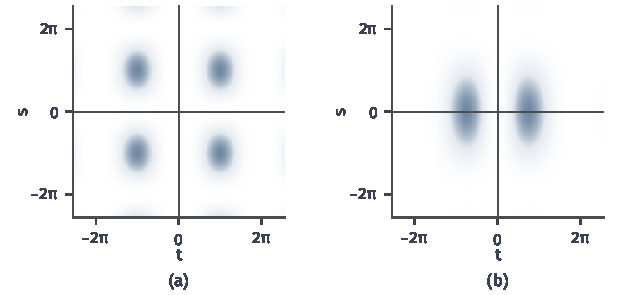
\includegraphics[width=108mm]{figures/07-probability/04-distribution-analysis/matplotlib/dep-cf-gap/figure.pdf}
  \caption{三点抛物线的特征函数之差。(a)$\lvert\Delta(t,s)\rvert^{2}=\frac{8}{81}(1-\cos t)^{2}(1-\cos s)$，白到蓝表示由小到大，在两条坐标轴上为零；(b)加权被积函数$\lvert\Delta\rvert^{2}/(\pi^{2}t^{2}s^{2})$，权重压低了高频，质量集中在$\lvert t\rvert\approx2$、$s$接近零的两块。(b)在全平面上的积分为$8/81$。}
  \label{fig:dep-cf-gap}
\end{BookInlineFigure}

\paragraph{权重不能随意替换}
零值判据的证明只用到权重处处为正与特征函数的唯一性；如果权重只在有界区域上为正，可能漏掉在那个区域外才出现的差别，因为两个不同的分布，其特征函数可以在一个区间上相同。权重的幂次也不能随意改动。若把$\lVert\bm{t}\rVert_2^{-(d+1)}$换成$\lVert\bm{t}\rVert_2^{-(d+\alpha)}$，引理的同样论证给出
\[
  \int_{\mathbb{R}^{d}}\frac{1-\cos\langle\bm{t},\bm{x}\rangle}{\lVert\bm{t}\rVert_2^{d+\alpha}}\,\mathrm{d}\bm{t}=c_{d,\alpha}\lVert\bm{x}\rVert_2^{\alpha},
\]
有限性要求原点附近$\lVert\bm{t}\rVert_2^{2-d-\alpha}$可积，即$\alpha<2$，无穷远处$\lVert\bm{t}\rVert_2^{-d-\alpha}$可积，即$\alpha>0$。所以$0<\alpha<2$时得到以$\lVert\bm{x}-\bm{x}'\rVert_2^{\alpha}$代替距离的一族度量，需要$\alpha$阶矩；$\alpha=2$时积分发散，下一小节会看到，强行把距离换成平方距离，零值判据就失效了。

\subsection{成对距离的表示}
\label{sec:dep-dcov-pairwise}

式~\eqref{eq:dep-dcov-def}是频率空间里的积分，实际计算时我们更希望回到取值空间。引理~\ref{lem:dep-cos-integral}已经把$1-\cos$换成距离，剩下的工作是把$\lvert\Delta\rvert^{2}$展开成若干个$1-\cos$的期望。为此引入$(\bm{X},\bm{Y})$的两个独立复制$(\bm{X}',\bm{Y}')$与$(\bm{X}'',\bm{Y}'')$，三组相互独立、同分布。

\begin{theorem}[距离协方差的成对距离表示]
\label{thm:dep-dcov-pairwise}
设$\mathbb{E}\lVert\bm{X}\rVert_2^{2}<\infty$，$\mathbb{E}\lVert\bm{Y}\rVert_2^{2}<\infty$。记$a=\lVert\bm{X}-\bm{X}'\rVert_2$，$b=\lVert\bm{Y}-\bm{Y}'\rVert_2$，$b''=\lVert\bm{Y}-\bm{Y}''\rVert_2$。则
\begin{equation}
  \operatorname{dCov}^{2}(\bm{X},\bm{Y})=\mathbb{E}[ab]+\mathbb{E}[a]\,\mathbb{E}[b]-2\,\mathbb{E}[ab''] .
  \label{eq:dep-dcov-pairwise}
\end{equation}
\end{theorem}

\begin{proof}
固定$(\bm{t},\bm{s})$，记三个随机相位
\[
  \theta=\langle\bm{t},\bm{X}-\bm{X}'\rangle,\qquad \eta=\langle\bm{s},\bm{Y}-\bm{Y}'\rangle,\qquad \eta''=\langle\bm{s},\bm{Y}-\bm{Y}''\rangle .
\]
用独立复制把$\lvert\Delta\rvert^{2}=\Delta\overline{\Delta}$的四项写成期望：
\[
  \begin{aligned}
    \phi_{\bm{X},\bm{Y}}\overline{\phi_{\bm{X},\bm{Y}}}&=\mathbb{E}\,\mathrm{e}^{\mathrm{i}(\theta+\eta)},\qquad
    \lvert\phi_{\bm{X}}\phi_{\bm{Y}}\rvert^{2}=\mathbb{E}\,\mathrm{e}^{\mathrm{i}\theta}\ \mathbb{E}\,\mathrm{e}^{\mathrm{i}\eta},\\
    \phi_{\bm{X},\bm{Y}}\overline{\phi_{\bm{X}}\phi_{\bm{Y}}}&=\mathbb{E}\,\mathrm{e}^{\mathrm{i}(\theta+\eta'')} .
  \end{aligned}
\]
第三项中$\overline{\phi_{\bm{X}}(\bm{t})}$用第二组复制写成期望，$\overline{\phi_{\bm{Y}}(\bm{s})}$用第三组复制。第四项是第三项的共轭。$\theta$与$-\theta$同分布，所以$\mathbb{E}\sin\theta=0$，同理$\mathbb{E}\sin\eta=0$。取实部，
\[
  \lvert\Delta\rvert^{2}=\mathbb{E}\cos\theta\cos\eta+\mathbb{E}\cos\theta\,\mathbb{E}\cos\eta-2\,\mathbb{E}\cos\theta\cos\eta''+S(\bm{t},\bm{s}),
\]
其中正弦部分为
\[
  S(\bm{t},\bm{s})=-\mathbb{E}\sin\theta\sin\eta+2\,\mathbb{E}\sin\theta\sin\eta'' .
\]

把$\cos\theta\cos\eta$写成$1-(1-\cos\theta)-(1-\cos\eta)+(1-\cos\theta)(1-\cos\eta)$，对另外两项同样展开。$\eta$与$\eta''$同分布，三项中常数与单个$1-\cos$的部分按系数$1+1-2=0$全部抵消。记$G(\bm{t},\bm{s})$为剩下的部分，
\[
  \begin{aligned}
  G={}&\mathbb{E}\bigl[(1-\cos\theta)(1-\cos\eta)\bigr]+\mathbb{E}[1-\cos\theta]\,\mathbb{E}[1-\cos\eta]\\
  &-2\,\mathbb{E}\bigl[(1-\cos\theta)(1-\cos\eta'')\bigr],
  \end{aligned}
\]
于是$\lvert\Delta\rvert^{2}=G+S$。

$S$关于$\bm{t}$是奇函数（$\bm{t}\to-\bm{t}$时$\sin\theta$变号），$G$是偶函数。权重关于$\bm{t}$对称，用代换$\bm{t}\to-\bm{t}$把式~\eqref{eq:dep-dcov-def}写成$\frac12(\lvert\Delta(\bm{t},\bm{s})\rvert^{2}+\lvert\Delta(-\bm{t},\bm{s})\rvert^{2})$的积分，这个平均正好是$G$。这一步只涉及非负函数的积分，不需要$S$可积。所以
\[
  \operatorname{dCov}^{2}(\bm{X},\bm{Y})=\frac{1}{c_pc_q}\int_{\mathbb{R}^{p+q}}\frac{G(\bm{t},\bm{s})}{\lVert\bm{t}\rVert_2^{p+1}\lVert\bm{s}\rVert_2^{q+1}}\,\mathrm{d}\bm{t}\,\mathrm{d}\bm{s}.
\]

$G$的三项各自是非负函数的期望。对第一项用Tonelli定理交换期望与积分，两次运用引理~\ref{lem:dep-cos-integral}，
\[
  \frac{1}{c_pc_q}\int\!\!\int\frac{\mathbb{E}[(1-\cos\theta)(1-\cos\eta)]}{\lVert\bm{t}\rVert_2^{p+1}\lVert\bm{s}\rVert_2^{q+1}}\,\mathrm{d}\bm{t}\,\mathrm{d}\bm{s}=\mathbb{E}[ab].
\]
第二、三项同理分别得到$\mathbb{E}[a]\mathbb{E}[b]$与$\mathbb{E}[ab'']$。由Cauchy--Schwarz不等式，$\mathbb{E}[ab]$不超过$(\mathbb{E}a^{2}\,\mathbb{E}b^{2})^{1/2}$，而由三角不等式$\mathbb{E}a^{2}$不超过$4\,\mathbb{E}\lVert\bm{X}\rVert_2^{2}$，是有限的，三项都有限，可以按线性逐项积分，得到式~\eqref{eq:dep-dcov-pairwise}。
\end{proof}

\paragraph{为什么需要二阶矩}
定义~\ref{def:dep-dcov}只需要一阶矩，式~\eqref{eq:dep-dcov-pairwise}却要求三项分别有限。只有一阶矩时，左边仍有限，右边可能是$\infty-\infty$。取$Y=X$，$X$服从第~\ref{chap:laws-of-large-numbers}章用过的$\alpha=1.5$的Pareto分布，$\mathbb{E}\lvert X\rvert<\infty$而$\mathbb{E}X^{2}=\infty$。这时$\mathbb{E}[ab]$就是$\mathbb{E}\lvert X-X'\rvert^{2}=\infty$，$\mathbb{E}[ab'']$也是无穷大，式~\eqref{eq:dep-dcov-pairwise}右边没有意义；而由式~\eqref{eq:dep-dcov-bound}，左边不超过$(\mathbb{E}\lvert X-X'\rvert)^{2}$，是有限的。二阶矩是让逐项展开合法的充分条件，不是距离协方差存在的条件。

\paragraph{双重中心化}
式~\eqref{eq:dep-dcov-pairwise}还可以写成一个“协方差”的样子。记$m(\bm{x})=\mathbb{E}\lVert\bm{x}-\bm{X}'\rVert_2$为点$\bm{x}$到$\bm{X}$的平均距离，$D=\mathbb{E}\lVert\bm{X}-\bm{X}'\rVert_2$。对成对距离作\term{双重中心化}（double centering），
\begin{equation}
  A(\bm{x},\bm{x}')=\lVert\bm{x}-\bm{x}'\rVert_2-m(\bm{x})-m(\bm{x}')+D ,
  \label{eq:dep-double-centering}
\end{equation}
即减去两端各自的平均距离，再加回总平均。对$\bm{Y}$同样定义$B(\bm{y},\bm{y}')$。则在定理~\ref{thm:dep-dcov-pairwise}的条件下
\begin{equation}
  \operatorname{dCov}^{2}(\bm{X},\bm{Y})=\mathbb{E}\bigl[A(\bm{X},\bm{X}')\,B(\bm{Y},\bm{Y}')\bigr].
  \label{eq:dep-dcov-centered}
\end{equation}

验证如下。记$n,D_Y$为$\bm{Y}$一侧与$m,D$对应的量。固定$\bm{y}$，对$\bm{Y}'$取期望，
\[
  \mathbb{E}\,B(\bm{y},\bm{Y}')=n(\bm{y})-n(\bm{y})-D_Y+D_Y=0 .
\]所以在$A$的四项中，只依赖$(\bm{X},\bm{Y})$一组的$m(\bm{X})$，与$B(\bm{Y},\bm{Y}')$相乘后先对$(\bm{X}',\bm{Y}')$取期望，得到零；$m(\bm{X}')$与常数$D$同理。只剩
\[
  \mathbb{E}\bigl[a\,B(\bm{Y},\bm{Y}')\bigr]=\mathbb{E}[ab]-\mathbb{E}\bigl[a\,n(\bm{Y})\bigr]-\mathbb{E}\bigl[a\,n(\bm{Y}')\bigr]+\mathbb{E}[a]\,D_Y .
\]
$n(\bm{Y})$是$b''$在给定$\bm{Y}$时的条件期望，所以$\mathbb{E}[a\,n(\bm{Y})]=\mathbb{E}[ab'']$；交换两组复制的角色，$\mathbb{E}[a\,n(\bm{Y}')]$也等于$\mathbb{E}[ab'']$。代回去就是式~\eqref{eq:dep-dcov-pairwise}的右边。

式~\eqref{eq:dep-dcov-centered}给出了一个直观的读法。$A(\bm{X},\bm{X}')>0$表示这一对$\bm{X}$比按各自位置预期的更远，$B>0$表示这一对$\bm{Y}$更远；距离协方差问的是“$\bm{X}$这对远时$\bm{Y}$这对是否也远”。中心化消去了只由一个边缘决定的部分：$m(\bm{x})$大只说明$\bm{x}$处在边缘分布的外围，与$\bm{Y}$无关。若$\bm{X},\bm{Y}$独立，则$(\bm{X},\bm{X}')$与$(\bm{Y},\bm{Y}')$独立，期望分解为$\mathbb{E}A\cdot\mathbb{E}B=0$。

\paragraph{平方距离只剩协方差}
现在可以看清为什么不能用平方距离。对实值变量把$\lvert x-x'\rvert$换成$(x-x')^{2}$，记$\mu=\mathbb{E}X$。$(x-x')^{2}$的平均是$m_2(x)=(x-\mu)^{2}+\operatorname{Var}(X)$，总平均是$2\operatorname{Var}(X)$，双重中心化后
\[
  (x-x')^{2}-m_2(x)-m_2(x')+2\operatorname{Var}(X)=-2(x-\mu)(x'-\mu).
\]
代入式~\eqref{eq:dep-dcov-centered}的形式，两组复制独立，
\[
  4\,\mathbb{E}\bigl[(X-\mu)(Y-\nu)(X'-\mu)(Y'-\nu)\bigr]=4\operatorname{Cov}(X,Y)^{2},
\]
其中$\nu=\mathbb{E}Y$。平方距离只保留了协方差，抛物线上为零；正是指数$1<2$使距离协方差看到了非线性的依赖。

\paragraph{三点抛物线的成对距离}
用式~\eqref{eq:dep-dcov-pairwise}重算三点抛物线。三个点的$x$坐标为$-1,0,1$，$y$坐标为$1,0,1$，成对距离矩阵为
\[
  \bm{A}=\begin{pmatrix}0&1&2\\1&0&1\\2&1&0\end{pmatrix},\qquad
  \bm{B}=\begin{pmatrix}0&1&0\\1&0&1\\0&1&0\end{pmatrix}.
\]
三点等可能，期望就是对$9$个元素求平均。第一项$\mathbb{E}[ab]$只在$\bm{B}$非零的四个位置有贡献，那里$\bm{A}$的元素都是$1$，
\[
  \mathbb{E}[ab]=\tfrac49,\qquad \mathbb{E}[a]=\tfrac89,\qquad \mathbb{E}[b]=\tfrac49 .
\]

第三项要先求每个点的平均距离：$\bm{A}$的行平均是$m=(1,\frac23,1)$，$\bm{B}$的行平均是$n=(\frac13,\frac23,\frac13)$。由$\mathbb{E}[ab'']=\mathbb{E}[m(X)\,n(Y)]$，
\[
  \mathbb{E}[ab'']=\tfrac13\Bigl(1\cdot\tfrac13+\tfrac23\cdot\tfrac23+1\cdot\tfrac13\Bigr)=\tfrac{10}{27}.
\]
代入式~\eqref{eq:dep-dcov-pairwise}，
\[
  \operatorname{dCov}^{2}(X,Y)=\frac49+\frac89\cdot\frac49-2\cdot\frac{10}{27}=\frac{36+32-60}{81}=\frac{8}{81},
\]
与特征函数积分的结果一致。

图~\ref{fig:dep-double-centering}给出双重中心化后的矩阵$\tilde{\bm{A}}$、$\tilde{\bm{B}}$：每行每列之和为零。按式~\eqref{eq:dep-dcov-centered}逐格相乘求和，
\[
  \frac19\sum_{i,j}\tilde{A}_{i,j}\tilde{B}_{i,j}=\frac19\cdot\frac{72}{81}=\frac{8}{81}.
\]

\begin{BookInlineFigure}
  \centering
  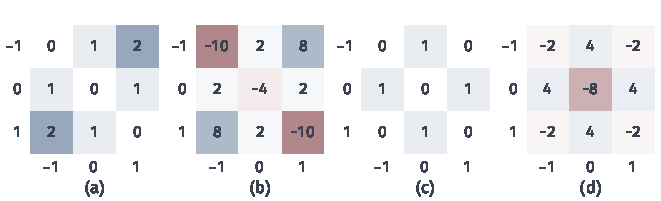
\includegraphics[width=112mm]{figures/07-probability/04-distribution-analysis/matplotlib/dep-double-centering/figure.pdf}
  \caption{三点抛物线的成对距离与双重中心化，行列按$x=-1,0,1$排列。(a)$\bm{A}=(\lvert x_i-x_j\rvert)$；(b)$\tilde{\bm{A}}$，格中数字乘以$1/9$；(c)$\bm{B}=(\lvert y_i-y_j\rvert)$；(d)$\tilde{\bm{B}}$，格中数字乘以$1/9$。(a)(c)白到蓝表示由小到大，(b)(d)红—白—蓝表示由负到正。中心化后每行每列之和为零。}
  \label{fig:dep-double-centering}
\end{BookInlineFigure}

$n$个样本点的经验分布也是这样一个等可能的有限分布，把式~\eqref{eq:dep-dcov-pairwise}用在经验分布上，就得到样本距离协方差。它作为总体量估计的性质，属于统计推断的问题。

\subsection{距离相关}
\label{sec:dep-dcor}

距离协方差有量纲：把$\bm{Y}$的单位从米换成厘米，$\operatorname{dCov}^{2}$乘以$100$。与由协方差得到相关系数一样，用各自的“距离方差”归一化。

\begin{definition}[距离相关]
\label{def:dep-dcor}
在定义~\ref{def:dep-dcov}的条件下，称$\bm{X}$与自身的距离协方差$\operatorname{dCov}^{2}(\bm{X},\bm{X})$为$\bm{X}$的\term{距离方差}（distance variance），记为$\operatorname{dVar}^{2}(\bm{X})$。$\bm{X}$与$\bm{Y}$的\term{距离相关}（distance correlation）定义为
\begin{equation}
  \operatorname{dCor}(\bm{X},\bm{Y})=
  \begin{cases}
    \dfrac{\operatorname{dCov}(\bm{X},\bm{Y})}{\sqrt{\operatorname{dVar}(\bm{X})\operatorname{dVar}(\bm{Y})}}, & \operatorname{dVar}(\bm{X})\operatorname{dVar}(\bm{Y})>0,\\
    0, & \operatorname{dVar}(\bm{X})\operatorname{dVar}(\bm{Y})=0 .
  \end{cases}
  \label{eq:dep-dcor}
\end{equation}
\end{definition}

第二行的约定只在常量情形起作用。由定理~\ref{thm:dep-dcov-independence}，$\operatorname{dVar}^{2}(\bm{X})=0$当且仅当$\bm{X}$与自身独立；这时对每个Borel集$C$，事件$\{\bm{X}\in C\}$与自身独立，它的概率$r$满足$r=r^{2}$，只能是$0$或$1$，每个坐标的分布函数只取$0,1$两个值，$\bm{X}$几乎必然是常数。常数与任何变量都独立，取距离相关为$0$与零值判据相容。

\begin{theorem}[距离相关的范围与不变性]
\label{thm:dep-dcor-properties}
在定义~\ref{def:dep-dcor}的条件下：
\begin{enumerate}
  \item $0\leq\operatorname{dCor}(\bm{X},\bm{Y})\leq1$，并且$\operatorname{dCor}(\bm{X},\bm{Y})=0$当且仅当$\bm{X}$与$\bm{Y}$独立；
  \item 对向量$\bm{a}_1\in\mathbb{R}^{p}$、$\bm{a}_2\in\mathbb{R}^{q}$，非零标量$b_1,b_2$与正交矩阵$\bm{C}_1,\bm{C}_2$，
  \begin{equation}
    \operatorname{dCov}^{2}(\bm{a}_1+b_1\bm{C}_1\bm{X},\ \bm{a}_2+b_2\bm{C}_2\bm{Y})=\lvert b_1b_2\rvert\operatorname{dCov}^{2}(\bm{X},\bm{Y}),
    \label{eq:dep-dcov-scaling}
  \end{equation}
  从而距离相关在这类变换下不变。
\end{enumerate}
\end{theorem}

\begin{proof}
零值部分由定理~\ref{thm:dep-dcov-independence}与常量约定直接得到。上界先在二阶矩有限时证明。由式~\eqref{eq:dep-dcov-centered}与Cauchy--Schwarz不等式，
\[
  \operatorname{dCov}^{2}(\bm{X},\bm{Y})\leq\bigl(\mathbb{E}A^{2}\bigr)^{1/2}\bigl(\mathbb{E}B^{2}\bigr)^{1/2}=\operatorname{dVar}(\bm{X})\operatorname{dVar}(\bm{Y}),
\]
最后一步对$\bm{Y}=\bm{X}$与$\bm{X}=\bm{Y}$再用一次式~\eqref{eq:dep-dcov-centered}。两边开方，除以$\operatorname{dVar}(\bm{X})\operatorname{dVar}(\bm{Y})$，得$\operatorname{dCor}\leq1$。

对第二部分，记$\bm{X}^{*}=\bm{a}_1+b_1\bm{C}_1\bm{X}$，它的特征函数为
\[
  \phi_{\bm{X}^{*}}(\bm{t})=\mathrm{e}^{\mathrm{i}\langle\bm{t},\bm{a}_1\rangle}\phi_{\bm{X}}\bigl(b_1\bm{C}_1^{\top}\bm{t}\bigr),
\]
联合特征函数同理。平移因子的模为$1$，所以变换后的差$\Delta^{*}$满足
\[
  \lvert\Delta^{*}(\bm{t},\bm{s})\rvert=\bigl\lvert\Delta\bigl(b_1\bm{C}_1^{\top}\bm{t},\,b_2\bm{C}_2^{\top}\bm{s}\bigr)\bigr\rvert .
\]
在式~\eqref{eq:dep-dcov-def}中作代换$\bm{u}=b_1\bm{C}_1^{\top}\bm{t}$。体积元变为$\lvert b_1\rvert^{-p}\mathrm{d}\bm{u}$，分母变为$\lvert b_1\rvert^{-p-1}\lVert\bm{u}\rVert_2^{p+1}$，积分多出因子$\lvert b_1\rvert$。$\bm{s}$一侧同样多出$\lvert b_2\rvert$，这就是式~\eqref{eq:dep-dcov-scaling}。对$\operatorname{dVar}^{2}$分别多出$b_1^{2}$与$b_2^{2}$，代入式~\eqref{eq:dep-dcor}相消。
\end{proof}

上界的证明用到了二阶矩。只有一阶矩时上界同样成立，需要先截断再验证各项的连续性，篇幅较长，可查阅\scite{math-szekely2007dependence}。

距离相关取到$1$的情形也已清楚：$\operatorname{dCor}(\bm{X},\bm{Y})=1$当且仅当$\bm{Y}=\bm{a}+b\bm{C}\bm{X}$几乎必然成立，其中$b\neq0$为标量、$\bm{C}$为正交矩阵，证明见同一文献。所以距离相关为$1$意味着两组坐标只差一个相似变换，比“$\bm{Y}$由$\bm{X}$确定”严格得多。

\paragraph{三点抛物线与高斯}
三点抛物线的距离方差由图~\ref{fig:dep-double-centering}的矩阵算出。中心化一侧即可，
\[
  \operatorname{dVar}^{2}(X)=\frac19\sum_{i,j}\tilde{A}_{i,j}A_{i,j}=\frac{40}{81},\qquad \operatorname{dVar}^{2}(Y)=\frac19\sum_{i,j}\tilde{B}_{i,j}B_{i,j}=\frac{16}{81}.
\]代入式~\eqref{eq:dep-dcor}，
\[
  \operatorname{dCor}^{2}(X,Y)=\frac{8/81}{\sqrt{(40/81)(16/81)}}=\frac{8}{\sqrt{640}}=\frac{1}{\sqrt{10}},
\]
所以$\operatorname{dCor}(X,Y)=10^{-1/4}\approx0.562$。$Y$由$X$确定，距离相关却远小于$1$，因为$Y=X^{2}$不是$X$的相似变换。

同一文献还算出了标准二元高斯的闭式结果：
\[
  \operatorname{dCor}^{2}=\frac{\rho\arcsin\rho+\sqrt{1-\rho^{2}}-\rho\arcsin(\rho/2)-\sqrt{4-\rho^{2}}+1}{1+\pi/3-\sqrt3}.
\]
$\rho=0.5$时约为$0.206$，即$\operatorname{dCor}\approx0.454$。图~\ref{fig:dep-dcor-gaussian}显示距离相关在高斯族内随$\lvert\rho\rvert$单调增，略低于$\lvert\rho\rvert$，两端与之重合。在高斯族内两者给出相同的次序，只是刻度不同。

\begin{BookInlineFigure}
  \centering
  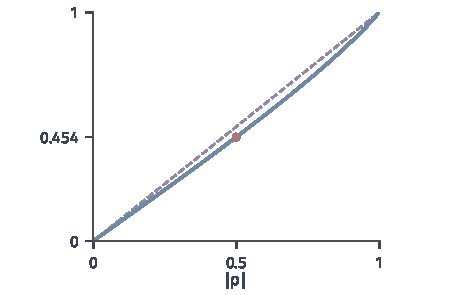
\includegraphics[width=80mm]{figures/07-probability/04-distribution-analysis/matplotlib/dep-dcor-gaussian/figure.pdf}
  \caption{标准二元高斯的距离相关随$\lvert\rho\rvert$的变化（蓝，闭式公式；脚本另用$60\times60$个Gauss--Hermite节点数值核对，相对误差在$0.3\%$以内）。紫色虚线是参考线$\lvert\rho\rvert$。红点为$\rho=0.5$处的$0.454$。}
  \label{fig:dep-dcor-gaussian}
\end{BookInlineFigure}

\paragraph{哪些变换保持距离相关}
定理~\ref{thm:dep-dcor-properties}允许的变换是平移、旋转（含反射）与同一个非零标量的整体缩放，它们保持距离之间的比例。其他变换一般会改变距离相关。把三点抛物线中$X$的取值$-1,0,1$改成$-1,0,5$，互信息不变，距离相关从$0.562$变为$0.530$。对高斯向量作坐标变换$(\mathrm{e}^{X},\mathrm{e}^{Y})$，距离相关从$0.454$变为约$0.42$；用$\Phi$变到Copula坐标，约为$0.45$；把$Y$整体乘以$10$则不变。图~\ref{fig:dep-transform-bars}把相关系数、距离相关与互信息放在一起比较：互信息在四种变换下都不动，距离相关只在相似变换下不动。若对$\bm{X}$的不同坐标用不同的比例缩放，例如$\operatorname{diag}(1,10)$，距离的比例被打乱，距离相关一般也会改变；多维时先统一各坐标的单位，再计算距离相关。

\begin{BookInlineFigure}
  \centering
  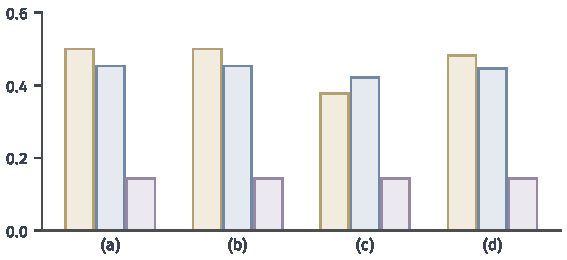
\includegraphics[width=96mm]{figures/07-probability/04-distribution-analysis/matplotlib/dep-transform-bars/figure.pdf}
  \caption{标准二元高斯（$\rho=0.5$）在四种坐标变换下的三个量：(a)原坐标；(b)$Y\mapsto10Y$；(c)$(\mathrm{e}^{X},\mathrm{e}^{Y})$；(d)$(\Phi(X),\Phi(Y))$。黄柱为相关系数的绝对值，蓝柱为距离相关（$90\times90$个Gauss--Hermite加权节点数值计算，约$0.453$、$0.453$、$0.422$、$0.445$），紫柱为互信息（nat，均为$0.144$）。}
  \label{fig:dep-transform-bars}
\end{BookInlineFigure}
